
\documentclass[template=tabling,81pt,headonall]{azmoon}
\usepackage{xepersian}
\usepackage{amsfonts}
\usepackage{graphicx}
\usepackage{svg}
\svgpath{ {./images/} }
\graphicspath{ {./images/} }
\settextfont{Yas}
\setdigitfont{A Iranian Sans}
\usepackage{fontawesome5}

\printanswers
    \teacher{محمد صالح علی اکبری}
    \teachertitle{دبیر}
    \city{گناباد}
    \schooltitle{دبیرستان}
    \school{شهید جوانبخت}
    \grade{هشتم (نمونه الف)}
    \branch{نمونه الف}
    \topic{ریاضی}
    \examdate{۲۳ مهر ۱۴۰۵}
    \answertime{۵۰ دقیقه}
    \begin{document}
	\begin{questions}
		\nointerlineskip%
		\vskip-\baselineskip
		\question[6]{%
\textbf{حاصل هر یک از عبارت‌های زیر را به دست آورید:}
\begin{LTR}
\begin{tabular*}{\linewidth}{@{\extracolsep{\fill}}lll}
الف) $25 + 34 = $ & ب) $84 - 29 = $ & ج) $120 + 230 = $ \\\\[0.5em]
د) $(-12) + (+7) = $ & هـ) $(-8) - (-15) = $ & و) $(-4) - (+9) + (-3) = $
\end{tabular*}
\end{LTR}}\question[4]{%
\textbf{به پرسش‌های زیر دربارهٔ عددهای گویا پاسخ دهید:}\\[0.2em]
الف) عددهای $-\dfrac{3}{4}$ و $+1\dfrac{1}{2}$ را روی محور زیر با رسم شکل یا علامت مشخص کنید:\\[0.15em]
\centerline{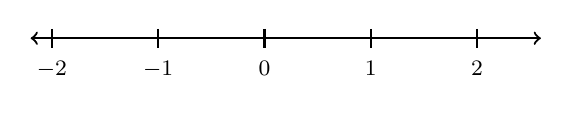
\begin{tikzpicture}[x=1.35cm]
\draw[<->,thick] (-2.2,0) -- (2.6,0);
\foreach \x in {-2,-1,0,1,2} \draw[thick] (\x,0.12) -- (\x,-0.12) node[below=1pt] {\footnotesize $\x$};
\end{tikzpicture}}\\[0.2em]
ب) قرینهٔ عدد $-\dfrac{5}{7}$ برابر است با: \dotfill \quad معکوس عدد $-\dfrac{2}{3}$ برابر است با: \dotfill \\\\[0.3em]
ج) آیا هر عدد صحیح یک عدد گویا است؟ با یک مثال توضیح دهید: \dotfill \\\\[0.3em]
د) در جای خالی علامت مناسب ($>$ یا $<$ یا $=$) قرار دهید: \hfill 
$-\dfrac{1}{2} \quad \bigcirc \quad -\dfrac{3}{4}$}\question[5]{%
\textbf{حاصل جمع و تفریق‌های زیر را به دست آورده و در صورت امکان ساده کنید:}
\begin{LTR}
\begin{tabular*}{\linewidth}{@{\extracolsep{\fill}}lll}
الف) $\left(-\dfrac{3}{5}\right) + \left(+\dfrac{1}{5}\right) = $ & 
ب) $\left(-\dfrac{2}{3}\right) - \left(+\dfrac{1}{4}\right) = $ & 
ج) $2 - \dfrac{3}{7} = $
\end{tabular*}
\end{LTR}‌
\\‌
\\}\question[5]{%
\textbf{حاصل عبارت‌های زیر را به دست آورید:}
\begin{LTR}
\begin{tabular*}{\linewidth}{@{\extracolsep{\fill}}ll}
الف) $\left(-\dfrac{4}{9}\right) \times \left(+\dfrac{3}{8}\right) = $ & 
ب) $\left(-\dfrac{6}{5}\right) \div \left(-\dfrac{3}{10}\right) = $ \\\\[1.8em]
\multicolumn{2}{l}{ج) $\left(-\dfrac{1}{2} + \dfrac{1}{3}\right) \times (-6) = $}
\end{tabular*}
\end{LTR}‌
\\}\end{questions}
    \end{document}
    